\chapter{Banco de Dados}

Os bancos de dados desempenham papel fundamental nos sistemas de informação, pois permitem armazenar, organizar e recuperar informações necessárias às atividades de uma organização. Segundo \textcite{Machado2020}, sua estrutura deve representar os dados de forma coerente com o domínio da aplicação, possibilitando consultas e atualizações que preservem a consistência das informações.

No modelo relacional, os dados são organizados em tabelas formadas por linhas e colunas. As linhas representam os registros armazenados, enquanto as colunas definem seus atributos. A identificação dos registros e a associação entre tabelas são estabelecidas por chaves primárias e estrangeiras, acompanhadas de restrições de integridade \parencite{Silberschatz2012}.

A definição do esquema envolve a escolha dos tipos de dados, da obrigatoriedade dos campos e das regras de relacionamento. Essas decisões determinam como as informações serão representadas e quais condições deverão ser respeitadas durante sua manipulação. Uma estrutura adequada contribui para reduzir inconsistências, preservar referências e apoiar a manutenção da aplicação.

No Civitas, o armazenamento utiliza PostgreSQL, enquanto o acesso aos dados é realizado com Entity Framework Core e o provedor Npgsql. A estrutura relaciona os cadastros administrativos às unidades consumidoras, aos orçamentos e às despesas, além de manter informações de usuários, auditoria, mensagens e recuperação de senha.

\section{Modelo Entidade-Relacionamento}

O Modelo Entidade-Relacionamento permite representar os elementos relevantes de um domínio, seus atributos e as associações existentes entre eles. Essa representação auxilia a compreensão das informações que precisam ser armazenadas e das dependências entre os registros. As cardinalidades indicam quantas ocorrências de uma entidade podem se relacionar com ocorrências de outra, contribuindo para a definição das restrições do modelo \parencite{Silberschatz2012}.

A transformação dessa organização para o modelo relacional resulta em tabelas, chaves e restrições. Nos relacionamentos de um para muitos, a referência é normalmente mantida por uma chave estrangeira na tabela correspondente ao lado de muitos. A nulabilidade e a unicidade das colunas também participam da definição das condições permitidas pelo banco.

A Figura~\ref{fig:diagrama-banco-civitas} apresenta o diagrama do banco de dados do Civitas, reunindo as tabelas, seus atributos e as ligações entre elas. Essa representação oferece uma visão geral da organização dos dados e auxilia a compreensão dos relacionamentos entre os cadastros administrativos, as unidades consumidoras, os orçamentos e as despesas. Os scripts SQL apresentados na Seção~\ref{sec:scripts-tabelas} complementam essa visão, detalhando as definições e as restrições da estrutura documentada.

\begin{figure}[p]
    \centering
    \caption{Diagrama do banco de dados do Civitas}
    \label{fig:diagrama-banco-civitas}
    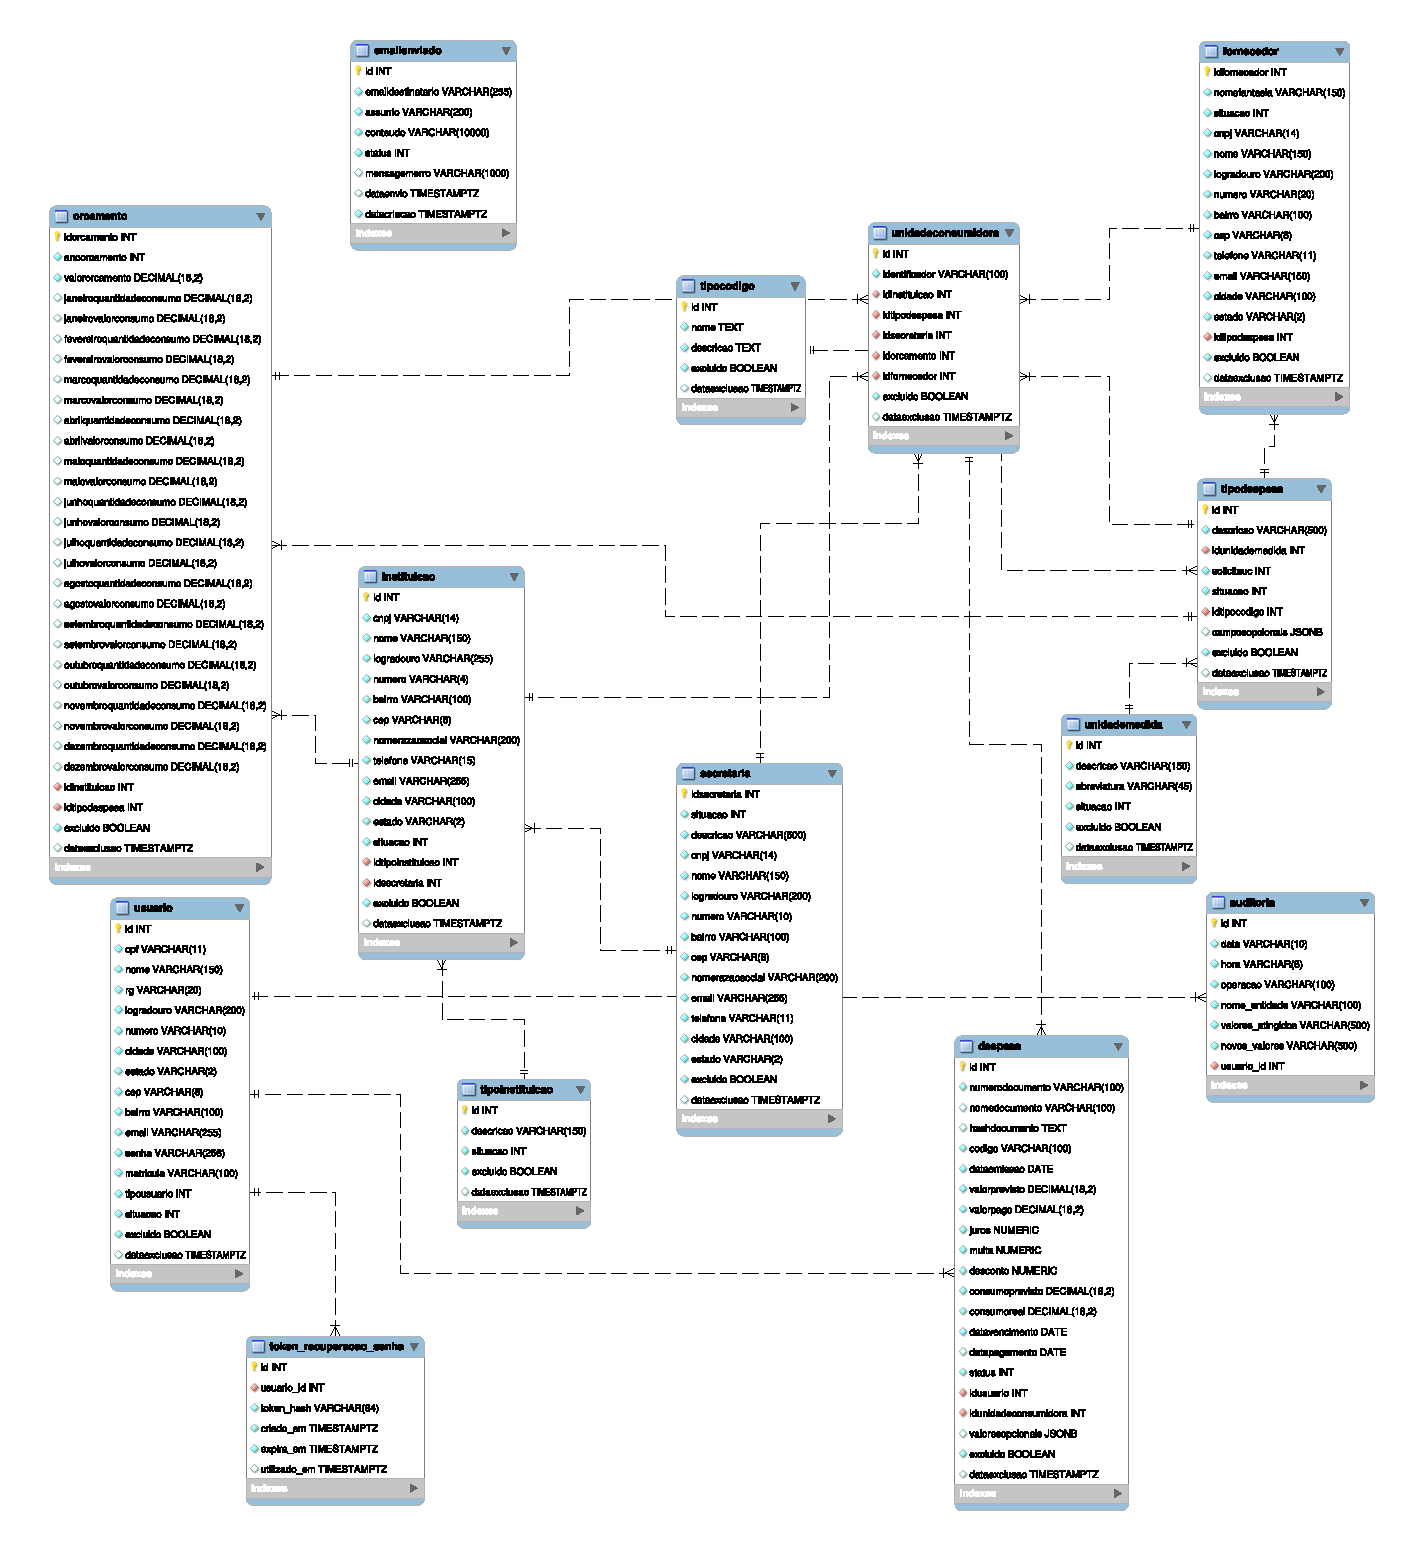
\includegraphics[width=\textwidth,height=0.82\textheight,keepaspectratio]{figs/civitas-eer-postgresql.pdf}
    \fonte{Elaborada pelos autores.}
\end{figure}

A estrutura administrativa é representada pelas tabelas secretaria, instituicao e tipoinstituicao. Cada instituição referencia uma secretaria e um tipo de instituição, enquanto cada registro dessas tabelas pode estar associado a nenhuma ou várias instituições.

Os cadastros auxiliares incluem unidademedida, tipocodigo e tipodespesa. Cada tipo de despesa referencia uma unidade de medida e um tipo de código. A tabela fornecedor também possui referência a tipodespesa, mantendo a associação entre o cadastro do fornecedor e sua classificação no sistema.

O planejamento financeiro é representado por orcamento, associado a instituicao e tipodespesa. Essa tabela armazena o exercício, o valor do orçamento e os campos de quantidade e valor de consumo previstos para os doze meses do ano. Os campos mensais admitem valores nulos, conforme a implementação examinada.

A tabela unidadeconsumidora estabelece referências à instituição, ao tipo de despesa, à secretaria, ao orçamento e ao fornecedor. Essas referências são obrigatórias em cada unidade consumidora. O campo identificador é obrigatório em cada registro da tabela.

As despesas possuem referências diretas ao usuário e à unidade consumidora. Dessa forma, fornecedor, instituição, orçamento e tipo de despesa são alcançados por meio da unidade consumidora, não constituindo chaves estrangeiras diretas da tabela despesa na estrutura examinada. Cada despesa referencia um usuário e uma unidade consumidora. Em sentido inverso, um usuário ou uma unidade consumidora pode estar associado a nenhuma ou várias despesas.

A tabela auditoria referencia usuario e mantém informações sobre operações. A tabela token\_recuperacao\_senha também está vinculada ao usuário e possui uma restrição para registros de tokens não utilizados. Já emailenviado armazena informações das mensagens sem possuir chave estrangeira nas migrations examinadas.

As ações de exclusão física variam conforme o relacionamento. A maioria das referências utiliza RESTRICT, enquanto as associações de tipodespesa com tipocodigo e de token\_recuperacao\_senha com usuario utilizam CASCADE. Essas ações não devem ser confundidas com exclusão lógica, representada pelos atributos excluido e dataexclusao nas tabelas que adotam esse mecanismo.

\section{Script das Tabelas}
\label{sec:scripts-tabelas}

Os scripts de definição de dados estabelecem a estrutura física do banco por meio de instruções SQL. O comando CREATE TABLE define tabelas, colunas e restrições de integridade. As definições devem corresponder à implementação, preservando nomes, tipos, nulabilidade e relacionamentos \parencite{Machado2020}.

Os scripts apresentados nesta seção foram organizados a partir das migrations do back-end do Civitas. A estrutura documentada considera a sequência de criação das tabelas e a alteração posterior identificada por \texttt{20261108032544\_remocao-campos-auditoria}, utilizada como referência para a apresentação do esquema.

Os Quadros 5.1 a 5.14 representam o estado final dessa sequência. Por isso, a tabela auditoria é apresentada sem os campos situacao, excluido e dataexclusao, removidos pela migration posterior. A forma varchar é utilizada como equivalente a character varying, mantendo os comprimentos declarados.

Os scripts constituem uma transcrição documental para criação de um esquema vazio, não um procedimento de atualização de banco existente. Não incluem dados de inicialização nem o histórico interno do Entity Framework Core e não foram executados em PostgreSQL durante esta revisão. A organização segue a ordem de dependência entre tabelas.

A tabela usuario reúne dados de identificação, endereço e acesso. CPF, e-mail e matrícula possuem índices únicos, enquanto tipousuario e situacao são armazenados como valores inteiros.

\begin{quadro}[H]
\caption{Script de criação da tabela usuario}\label{qua:bd-usuario}
\begin{lstlisting}[language=SQL,breaklines=true,breakatwhitespace=false,frame=single,columns=fullflexible,basicstyle=\ttfamily\footnotesize]
CREATE TABLE usuario (
    id integer GENERATED BY DEFAULT AS IDENTITY,
    cpf varchar(11) NOT NULL,
    nome varchar(150) NOT NULL,
    rg varchar(20) NOT NULL,
    logradouro varchar(200) NOT NULL,
    numero varchar(10) NOT NULL,
    cidade varchar(100) NOT NULL,
    estado varchar(2) NOT NULL,
    cep varchar(8) NOT NULL,
    bairro varchar(100) NOT NULL,
    email varchar(255) NOT NULL,
    senha varchar(256) NOT NULL,
    matricula varchar(100) NOT NULL,
    tipousuario integer NOT NULL,
    situacao integer NOT NULL,
    excluido boolean NOT NULL DEFAULT false,
    dataexclusao timestamp with time zone,
    CONSTRAINT "PK_usuario" PRIMARY KEY (id)
);
\end{lstlisting}
\fonte{Elaborado pelos autores com base nas migrations do back-end do Civitas.}
\end{quadro}

A tabela secretaria armazena informações dos órgãos administrativos. Sua chave primária utiliza o nome idsecretaria, preservado nas referências das tabelas relacionadas.

\begin{quadro}[H]
\caption{Script de criação da tabela secretaria}\label{qua:bd-secretaria}
\begin{lstlisting}[language=SQL,breaklines=true,breakatwhitespace=false,frame=single,columns=fullflexible,basicstyle=\ttfamily\footnotesize]
CREATE TABLE secretaria (
    idsecretaria integer GENERATED BY DEFAULT AS IDENTITY,
    situacao integer NOT NULL,
    descricao varchar(500) NOT NULL,
    cnpj varchar(14) NOT NULL,
    nome varchar(150) NOT NULL,
    logradouro varchar(200) NOT NULL,
    numero varchar(10) NOT NULL,
    bairro varchar(100) NOT NULL,
    cep varchar(8) NOT NULL,
    nomerazaosocial varchar(200) NOT NULL,
    email varchar(255) NOT NULL,
    telefone varchar(11) NOT NULL,
    cidade varchar(100) NOT NULL,
    estado varchar(2) NOT NULL,
    excluido boolean NOT NULL DEFAULT false,
    dataexclusao timestamp with time zone,
    CONSTRAINT "PK_secretaria" PRIMARY KEY (idsecretaria)
);
\end{lstlisting}
\fonte{Elaborado pelos autores com base nas migrations do back-end do Civitas.}
\end{quadro}

A tabela tipocodigo mantém as classificações de códigos utilizadas pelos tipos de despesa. Nome e descrição são armazenados como text, sem limite de comprimento declarado na migration.

\begin{quadro}[H]
\caption{Script de criação da tabela tipocodigo}\label{qua:bd-tipocodigo}
\begin{lstlisting}[language=SQL,breaklines=true,breakatwhitespace=false,frame=single,columns=fullflexible,basicstyle=\ttfamily\footnotesize]
CREATE TABLE tipocodigo (
    id integer GENERATED BY DEFAULT AS IDENTITY,
    nome text NOT NULL,
    descricao text NOT NULL,
    excluido boolean NOT NULL DEFAULT false,
    dataexclusao timestamp with time zone,
    CONSTRAINT "PK_tipocodigo" PRIMARY KEY (id)
);
\end{lstlisting}
\fonte{Elaborado pelos autores com base nas migrations do back-end do Civitas.}
\end{quadro}

A tabela unidademedida padroniza a descrição e a abreviatura das unidades utilizadas no sistema. A situação funcional é armazenada separadamente da marcação de exclusão lógica.

\begin{quadro}[H]
\caption{Script de criação da tabela unidademedida}\label{qua:bd-unidademedida}
\begin{lstlisting}[language=SQL,breaklines=true,breakatwhitespace=false,frame=single,columns=fullflexible,basicstyle=\ttfamily\footnotesize]
CREATE TABLE unidademedida (
    id integer GENERATED BY DEFAULT AS IDENTITY,
    descricao varchar(150) NOT NULL,
    abreviatura varchar(45) NOT NULL,
    situacao integer NOT NULL,
    excluido boolean NOT NULL DEFAULT false,
    dataexclusao timestamp with time zone,
    CONSTRAINT "PK_unidademedida" PRIMARY KEY (id)
);
\end{lstlisting}
\fonte{Elaborado pelos autores com base nas migrations do back-end do Civitas.}
\end{quadro}

A tabela tipoinstituicao representa as classificações das instituições. Um mesmo tipo pode ser referenciado por várias instituições.

\begin{quadro}[H]
\caption{Script de criação da tabela tipoinstituicao}\label{qua:bd-tipoinstituicao}
\begin{lstlisting}[language=SQL,breaklines=true,breakatwhitespace=false,frame=single,columns=fullflexible,basicstyle=\ttfamily\footnotesize]
CREATE TABLE tipoinstituicao (
    id integer GENERATED BY DEFAULT AS IDENTITY,
    descricao varchar(150) NOT NULL,
    situacao integer NOT NULL,
    excluido boolean NOT NULL DEFAULT false,
    dataexclusao timestamp with time zone,
    CONSTRAINT "PK_tipoinstituicao" PRIMARY KEY (id)
);
\end{lstlisting}
\fonte{Elaborado pelos autores com base nas migrations do back-end do Civitas.}
\end{quadro}

A tabela tipodespesa mantém a classificação, a unidade de medida, o tipo de código e as informações opcionais. O campo camposopcionais utiliza jsonb. A referência a tipocodigo possui ação CASCADE, enquanto a referência a unidademedida utiliza RESTRICT.

\begin{quadro}[H]
\caption{Script de criação da tabela tipodespesa}\label{qua:bd-tipodespesa}
\begin{lstlisting}[language=SQL,breaklines=true,breakatwhitespace=false,frame=single,columns=fullflexible,basicstyle=\ttfamily\footnotesize]
CREATE TABLE tipodespesa (
    id integer GENERATED BY DEFAULT AS IDENTITY,
    descricao varchar(500) NOT NULL,
    idunidademedida integer NOT NULL,
    solicitauc integer NOT NULL,
    situacao integer NOT NULL,
    idtipocodigo integer NOT NULL,
    camposopcionais jsonb,
    excluido boolean NOT NULL DEFAULT false,
    dataexclusao timestamp with time zone,
    CONSTRAINT "PK_tipodespesa" PRIMARY KEY (id),
    CONSTRAINT "FK_tipodespesa_tipocodigo_idtipocodigo"
        FOREIGN KEY (idtipocodigo) REFERENCES tipocodigo (id) ON DELETE CASCADE,
    CONSTRAINT "FK_tipodespesa_unidademedida_idunidademedida"
        FOREIGN KEY (idunidademedida) REFERENCES unidademedida (id) ON DELETE RESTRICT
);
\end{lstlisting}
\fonte{Elaborado pelos autores com base nas migrations do back-end do Civitas.}
\end{quadro}

A tabela fornecedor reúne dados cadastrais e referencia um tipo de despesa. A chave primária é identificada por idfornecedor.

\begin{quadro}[H]
\caption{Script de criação da tabela fornecedor}\label{qua:bd-fornecedor}
\begin{lstlisting}[language=SQL,breaklines=true,breakatwhitespace=false,frame=single,columns=fullflexible,basicstyle=\ttfamily\footnotesize]
CREATE TABLE fornecedor (
    idfornecedor integer GENERATED BY DEFAULT AS IDENTITY,
    nomefantasia varchar(150) NOT NULL,
    situacao integer NOT NULL,
    cnpj varchar(14) NOT NULL,
    nome varchar(150) NOT NULL,
    logradouro varchar(200) NOT NULL,
    numero varchar(20) NOT NULL,
    bairro varchar(100) NOT NULL,
    cep varchar(8) NOT NULL,
    telefone varchar(11) NOT NULL,
    email varchar(150) NOT NULL,
    cidade varchar(100) NOT NULL,
    estado varchar(2) NOT NULL,
    idtipodespesa integer NOT NULL,
    excluido boolean NOT NULL DEFAULT false,
    dataexclusao timestamp with time zone,
    CONSTRAINT "PK_fornecedor" PRIMARY KEY (idfornecedor),
    CONSTRAINT "FK_fornecedor_tipodespesa_idtipodespesa"
        FOREIGN KEY (idtipodespesa) REFERENCES tipodespesa (id) ON DELETE RESTRICT
);
\end{lstlisting}
\fonte{Elaborado pelos autores com base nas migrations do back-end do Civitas.}
\end{quadro}

A tabela instituicao mantém informações cadastrais e referências obrigatórias à secretaria e ao tipo de instituição. As duas chaves estrangeiras utilizam RESTRICT.

\begin{quadro}[H]
\caption{Script de criação da tabela instituicao}\label{qua:bd-instituicao}
\begin{lstlisting}[language=SQL,breaklines=true,breakatwhitespace=false,frame=single,columns=fullflexible,basicstyle=\ttfamily\footnotesize]
CREATE TABLE instituicao (
    id integer GENERATED BY DEFAULT AS IDENTITY,
    cnpj varchar(14) NOT NULL,
    nome varchar(150) NOT NULL,
    logradouro varchar(255) NOT NULL,
    numero varchar(4) NOT NULL,
    bairro varchar(100) NOT NULL,
    cep varchar(8) NOT NULL,
    nomerazaosocial varchar(200) NOT NULL,
    telefone varchar(15) NOT NULL,
    email varchar(255) NOT NULL,
    cidade varchar(100) NOT NULL,
    estado varchar(2) NOT NULL,
    situacao integer NOT NULL,
    idtipoinstituicao integer NOT NULL,
    idsecretaria integer NOT NULL,
    excluido boolean NOT NULL DEFAULT false,
    dataexclusao timestamp with time zone,
    CONSTRAINT "PK_instituicao" PRIMARY KEY (id),
    CONSTRAINT "FK_instituicao_secretaria_idsecretaria"
        FOREIGN KEY (idsecretaria) REFERENCES secretaria (idsecretaria) ON DELETE RESTRICT,
    CONSTRAINT "FK_instituicao_tipoinstituicao_idtipoinstituicao"
        FOREIGN KEY (idtipoinstituicao) REFERENCES tipoinstituicao (id) ON DELETE RESTRICT
);
\end{lstlisting}
\fonte{Elaborado pelos autores com base nas migrations do back-end do Civitas.}
\end{quadro}

A tabela orcamento armazena o exercício, o valor total e as previsões mensais de quantidade e valor de consumo. Os campos mensais admitem nulos, enquanto o exercício, o valor do orçamento e as referências são obrigatórios.

\begin{quadro}[H]
\caption{Script de criação da tabela orcamento}\label{qua:bd-orcamento}
\begin{lstlisting}[language=SQL,breaklines=true,breakatwhitespace=false,frame=single,columns=fullflexible,basicstyle=\ttfamily\footnotesize]
CREATE TABLE orcamento (
    idorcamento integer GENERATED BY DEFAULT AS IDENTITY,
    anoorcamento integer NOT NULL,
    valororcamento numeric(18,2) NOT NULL,
    janeiroquantidadeconsumo numeric(18,2), janeirovalorconsumo numeric(18,2),
    fevereiroquantidadeconsumo numeric(18,2), fevereirovalorconsumo numeric(18,2),
    marcoquantidadeconsumo numeric(18,2), marcovalorconsumo numeric(18,2),
    abrilquantidadeconsumo numeric(18,2), abrilvalorconsumo numeric(18,2),
    maioquantidadeconsumo numeric(18,2), maiovalorconsumo numeric(18,2),
    junhoquantidadeconsumo numeric(18,2), junhovalorconsumo numeric(18,2),
    julhoquantidadeconsumo numeric(18,2), julhovalorconsumo numeric(18,2),
    agostoquantidadeconsumo numeric(18,2), agostovalorconsumo numeric(18,2),
    setembroquantidadeconsumo numeric(18,2), setembrovalorconsumo numeric(18,2),
    outubroquantidadeconsumo numeric(18,2), outubrovalorconsumo numeric(18,2),
    novembroquantidadeconsumo numeric(18,2), novembrovalorconsumo numeric(18,2),
    dezembroquantidadeconsumo numeric(18,2), dezembrovalorconsumo numeric(18,2),
    idinstituicao integer NOT NULL,
    idtipodespesa integer NOT NULL,
    excluido boolean NOT NULL DEFAULT false,
    dataexclusao timestamp with time zone,
    CONSTRAINT "PK_orcamento" PRIMARY KEY (idorcamento),
    CONSTRAINT "FK_orcamento_instituicao_idinstituicao"
        FOREIGN KEY (idinstituicao) REFERENCES instituicao (id) ON DELETE RESTRICT,
    CONSTRAINT "FK_orcamento_tipodespesa_idtipodespesa"
        FOREIGN KEY (idtipodespesa) REFERENCES tipodespesa (id) ON DELETE RESTRICT
);
\end{lstlisting}
\fonte{Elaborado pelos autores com base nas migrations do back-end do Civitas.}
\end{quadro}

A tabela unidadeconsumidora possui cinco chaves estrangeiras. Na migration examinada, existe somente idfornecedor para a referência ao fornecedor, sem uma coluna adicional denominada FornecedorIdFornecedor.

\begin{quadro}[H]
\caption{Script de criação da tabela unidadeconsumidora}\label{qua:bd-unidadeconsumidora}
\begin{lstlisting}[language=SQL,breaklines=true,breakatwhitespace=false,frame=single,columns=fullflexible,basicstyle=\ttfamily\footnotesize]
CREATE TABLE unidadeconsumidora (
    id integer GENERATED BY DEFAULT AS IDENTITY,
    identificador varchar(100) NOT NULL,
    idinstituicao integer NOT NULL,
    idtipodespesa integer NOT NULL,
    idsecretaria integer NOT NULL,
    idorcamento integer NOT NULL,
    idfornecedor integer NOT NULL,
    excluido boolean NOT NULL DEFAULT false,
    dataexclusao timestamp with time zone,
    CONSTRAINT "PK_unidadeconsumidora" PRIMARY KEY (id),
    CONSTRAINT "FK_unidadeconsumidora_instituicao_idinstituicao"
        FOREIGN KEY (idinstituicao) REFERENCES instituicao (id) ON DELETE RESTRICT,
    CONSTRAINT "FK_unidadeconsumidora_tipodespesa_idtipodespesa"
        FOREIGN KEY (idtipodespesa) REFERENCES tipodespesa (id) ON DELETE RESTRICT,
    CONSTRAINT "FK_unidadeconsumidora_secretaria_idsecretaria"
        FOREIGN KEY (idsecretaria) REFERENCES secretaria (idsecretaria) ON DELETE RESTRICT,
    CONSTRAINT "FK_unidadeconsumidora_orcamento_idorcamento"
        FOREIGN KEY (idorcamento) REFERENCES orcamento (idorcamento) ON DELETE RESTRICT,
    CONSTRAINT "FK_unidadeconsumidora_fornecedor_idfornecedor"
        FOREIGN KEY (idfornecedor) REFERENCES fornecedor (idfornecedor) ON DELETE RESTRICT
);
\end{lstlisting}
\fonte{Elaborado pelos autores com base nas migrations do back-end do Civitas.}
\end{quadro}

A tabela despesa mantém informações documentais, financeiras e de consumo. As referências diretas são usuario e unidadeconsumidora. Juros, multa e desconto utilizam numeric sem precisão explícita, enquanto os campos de valores e consumos indicados utilizam numeric(18,2).

\begin{quadro}[H]
\caption{Script de criação da tabela despesa}\label{qua:bd-despesa}
\begin{lstlisting}[language=SQL,breaklines=true,breakatwhitespace=false,frame=single,columns=fullflexible,basicstyle=\ttfamily\footnotesize]
CREATE TABLE despesa (
    id integer GENERATED BY DEFAULT AS IDENTITY,
    numerodocumento varchar(100) NOT NULL,
    nomedocumento varchar(100),
    hashdocumento text,
    codigo varchar(100) NOT NULL,
    dataemissao date NOT NULL,
    valorprevisto numeric(18,2) NOT NULL,
    valorpago numeric(18,2) NOT NULL,
    juros numeric NOT NULL,
    multa numeric NOT NULL,
    desconto numeric NOT NULL,
    consumoprevisto numeric(18,2) NOT NULL,
    consumoreal numeric(18,2) NOT NULL,
    datavencimento date NOT NULL,
    datapagamento date,
    status integer NOT NULL,
    idusuario integer NOT NULL,
    idunidadeconsumidora integer NOT NULL,
    valoresopcionais jsonb,
    excluido boolean NOT NULL DEFAULT false,
    dataexclusao timestamp with time zone,
    CONSTRAINT "PK_despesa" PRIMARY KEY (id),
    CONSTRAINT "FK_despesa_unidadeconsumidora_idunidadeconsumidora"
        FOREIGN KEY (idunidadeconsumidora) REFERENCES unidadeconsumidora (id) ON DELETE RESTRICT,
    CONSTRAINT "FK_despesa_usuario_idusuario"
        FOREIGN KEY (idusuario) REFERENCES usuario (id) ON DELETE RESTRICT
);
\end{lstlisting}
\fonte{Elaborado pelos autores com base nas migrations do back-end do Civitas.}
\end{quadro}

A tabela auditoria é apresentada no estado posterior à remoção de situacao, excluido e dataexclusao. Data e hora permanecem campos textuais, conforme a implementação, sem conversão documental para tipos temporais.

\begin{quadro}[H]
\caption{Script de criação da tabela auditoria}\label{qua:bd-auditoria}
\begin{lstlisting}[language=SQL,breaklines=true,breakatwhitespace=false,frame=single,columns=fullflexible,basicstyle=\ttfamily\footnotesize]
CREATE TABLE auditoria (
    id integer GENERATED BY DEFAULT AS IDENTITY,
    data varchar(10) NOT NULL,
    hora varchar(8) NOT NULL,
    operacao varchar(100) NOT NULL,
    nome_entidade varchar(100) NOT NULL,
    valores_atingidos varchar(500) NOT NULL,
    novos_valores varchar(500) NOT NULL,
    usuario_id integer NOT NULL,
    CONSTRAINT "PK_auditoria" PRIMARY KEY (id),
    CONSTRAINT "FK_auditoria_usuario_usuario_id"
        FOREIGN KEY (usuario_id) REFERENCES usuario (id) ON DELETE RESTRICT
);
\end{lstlisting}
\fonte{Elaborado pelos autores com base nas migrations do back-end do Civitas, considerando a remoção dos campos de situação e exclusão lógica.}
\end{quadro}

A tabela emailenviado mantém destinatário, assunto, conteúdo e informações de envio. Mensagem de erro e data de envio são opcionais. Não há chave estrangeira definida nessa tabela.

\begin{quadro}[H]
\caption{Script de criação da tabela emailenviado}\label{qua:bd-emailenviado}
\begin{lstlisting}[language=SQL,breaklines=true,breakatwhitespace=false,frame=single,columns=fullflexible,basicstyle=\ttfamily\footnotesize]
CREATE TABLE emailenviado (
    id integer GENERATED BY DEFAULT AS IDENTITY,
    emaildestinatario varchar(255) NOT NULL,
    assunto varchar(200) NOT NULL,
    conteudo varchar(10000) NOT NULL,
    status integer NOT NULL,
    mensagemerro varchar(1000),
    dataenvio timestamp with time zone,
    datacriacao timestamp with time zone NOT NULL,
    CONSTRAINT "PK_emailenviado" PRIMARY KEY (id)
);
\end{lstlisting}
\fonte{Elaborado pelos autores com base nas migrations do back-end do Civitas.}
\end{quadro}

A tabela token\_recuperacao\_senha referencia usuario com ação CASCADE. A migration também define índices para o hash e para os tokens não utilizados; esses comandos não são reproduzidos nos scripts desta seção.

\begin{quadro}[H]
\caption{Script de criação da tabela token\_recuperacao\_senha}\label{qua:bd-token}
\begin{lstlisting}[language=SQL,breaklines=true,breakatwhitespace=false,frame=single,columns=fullflexible,basicstyle=\ttfamily\footnotesize]
CREATE TABLE token_recuperacao_senha (
    id integer GENERATED BY DEFAULT AS IDENTITY,
    usuario_id integer NOT NULL,
    token_hash varchar(64) NOT NULL,
    criado_em timestamp with time zone NOT NULL,
    expira_em timestamp with time zone NOT NULL,
    utilizado_em timestamp with time zone,
    CONSTRAINT "PK_token_recuperacao_senha" PRIMARY KEY (id),
    CONSTRAINT "FK_token_recuperacao_senha_usuario_usuario_id"
        FOREIGN KEY (usuario_id) REFERENCES usuario (id) ON DELETE CASCADE
);
\end{lstlisting}
\fonte{Elaborado pelos autores com base nas migrations do back-end do Civitas.}
\end{quadro}

\section{Mapeamento Objeto-Relacional}

O mapeamento objeto-relacional permite associar classes e propriedades da aplicação às tabelas e colunas de um banco relacional. Essa abordagem oferece uma camada de acesso aos dados na qual o desenvolvedor trabalha com objetos, enquanto o ORM participa da tradução das consultas e da persistência das alterações. Entity Framework Core fornece esse mecanismo no ecossistema .NET \parencite{MicrosoftEFCore}.

No Civitas, Entity Framework Core é integrado ao PostgreSQL pelo provedor Npgsql. A configuração ocorre em Program.cs, com o registro de AppDbContext e a utilização da conexão identificada por DefaultConnection. O trecho seguinte apresenta essa configuração, com as quebras de linha ajustadas para leitura:

\begin{verbatim}
builder.Services.AddDbContext<AppDbContext>(opt =>
{
    opt.UseNpgsql(
        builder.Configuration.GetConnectionString(
            "DefaultConnection"));
});
\end{verbatim}

AddDbContext registra o contexto no contêiner de dependências da aplicação. UseNpgsql seleciona o provedor de PostgreSQL e recebe a configuração de conexão. Essa composição permite que o contexto utilize o provedor correspondente ao sistema gerenciador adotado \parencite{MicrosoftDbContext}.

AppDbContext herda de DbContext e declara os conjuntos de entidades por propriedades DbSet. Entre esses conjuntos estão usuários, fornecedores, secretarias, instituições, orçamentos, unidades consumidoras e despesas, além das entidades auxiliares. Os nomes das propriedades não determinam isoladamente os nomes físicos das tabelas, pois o mapeamento também considera atributos e configurações explícitas.

As entidades utilizam atributos como Table e Column para identificar tabelas e colunas. As configurações complementares são estabelecidas por classes Builder, chamadas em OnModelCreating. Elas utilizam a Fluent API para definir chaves, comprimentos, obrigatoriedade, índices e relacionamentos.

Um exemplo está em UnidadeConsumidoraBuilder, que configura a associação com fornecedor:

\begin{verbatim}
modelBuilder.Entity<UnidadeConsumidora>()
    .HasOne(uc => uc.Fornecedor)
    .WithMany(x => x.UnidadesConsumidoras)
    .HasForeignKey(uc => uc.IdFornecedor)
    .OnDelete(DeleteBehavior.Restrict);
\end{verbatim}

HasOne identifica a referência da unidade consumidora ao fornecedor, enquanto WithMany indica a coleção inversa. HasForeignKey seleciona IdFornecedor como propriedade de referência, e OnDelete define a ação associada à exclusão física do registro principal.

A associação entre despesa e unidade consumidora é configurada em DespesaBuilder:

\begin{verbatim}
modelBuilder.Entity<Despesa>()
    .HasOne(d => d.UnidadeConsumidora)
    .WithMany(uc => uc.Despesas)
    .HasForeignKey(d => d.IdUnidadeConsumidora)
    .OnDelete(DeleteBehavior.Restrict);
\end{verbatim}

AppDbContext também percorre entidades que implementam ISoftDeletable e configura excluido e dataexclusao, incluindo o valor padrão false para o primeiro campo. Essa definição não constitui um filtro global de consulta. Nos métodos examinados do repositório genérico, a seleção dos registros é feita por um filtro aplicado pelo próprio repositório.

A interpretação dos Builders exige verificar quais configurações são efetivamente utilizadas. Embora TipoCodigoBuilder exista no projeto, ele não aparece entre as chamadas Build de OnModelCreating consultadas. A tabela continua presente nas migrations, e a entidade está exposta no contexto. Portanto, a existência de uma classe de configuração, isoladamente, não demonstra sua aplicação ao modelo.

As migrations registram alterações incrementais do esquema. O método Up descreve as operações de aplicação, enquanto Down apresenta operações de reversão. O snapshot representa o modelo utilizado para identificar alterações futuras, não o estado de uma instalação. Para determinar as migrations aplicadas, é necessário consultar o histórico do próprio banco \parencite{MicrosoftMigrations}.

As operações de consulta e persistência podem ser observadas em GenericRepository. O método Get utiliza uma consulta sem rastreamento, acompanhada do filtro de exclusão lógica quando aplicável:

\begin{verbatim}
return await ApplySoftDeleteFilter(
    _dbSet.AsNoTracking(),
    excluido: false
).ToListAsync();
\end{verbatim}

AsNoTracking evita o rastreamento das entidades retornadas por essa consulta. ApplySoftDeleteFilter aplica a seleção correspondente quando a entidade implementa ISoftDeletable, e ToListAsync materializa o resultado. A descrição corresponde à leitura do código, sem execução da consulta durante esta revisão.

No método Add, o repositório utiliza as seguintes chamadas:

\begin{verbatim}
await _dbSet.AddAsync(entity);
await SaveChanges();
\end{verbatim}

O método SaveChanges encaminha a gravação ao contexto por meio de SaveChangesAsync. AddAsync informa ao contexto a inclusão de uma entidade, enquanto SaveChangesAsync solicita a persistência das alterações acompanhadas. Portanto, a inclusão no conjunto não deve ser confundida com a conclusão da gravação no banco \parencite{MicrosoftSavingData}.

Na atualização, o repositório identifica a chave da entidade, trata uma possível instância já rastreada e utiliza EntityState.Modified antes de salvar. O método Remove realiza remoção física pelo conjunto, demonstrando que os campos de exclusão lógica não convertem automaticamente qualquer remoção em atualização.

O uso do ORM reduz a necessidade de SQL manual em operações recorrentes, mas não substitui as restrições do banco, as regras de negócio ou os testes. A estrutura apresentada corresponde ao código examinado. Sua reprodução e compatibilidade com um banco existente dependem de execução e verificação em ambiente apropriado.
